\begin{figure}[ht]
  \caption{diagram of different projects}
  \centering
  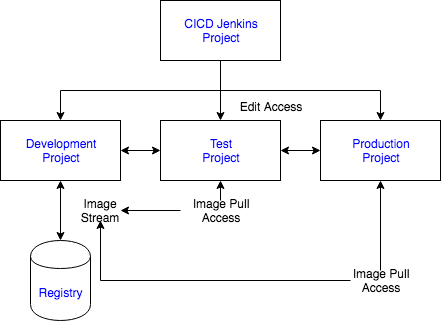
\includegraphics[scale=0.6]{ProjectPipelineDiagram.png}
  \label{fig:ProjectPipelineDiagram}
\end{figure}

\section{Build, Tag, Promote}

\paragraph{CICD}
Containing our Jenkins instance.

\paragraph{Development}
For building and developing our application images.

\paragraph{Testing}
For testing our application

\paragraph{Production}
Hosting our production application

\subsection{Create Projects}
\begin{minted}{bash}
  $ oc login -u developer -p developer
  $ oc new-project cicd --display-name='CICD Jenkins' \
  --description='CICD Jenkins'  
  $ oc new-project development --display-name='Development' \
  --description='Development'
  $ oc new-project testing --display-name='Testing' \
  --description='Testing'
  $ oc new-project production --display-name='Production' \
  --description='Production'  
\end{minted}

\subsection{Modify RBAC}

Let’s add in RBAC to our projects to allow the different service accounts to build, pro‐ mote, and tag images. First we will allow the cicd project’s Jenkins service account edit access to all of our projects:

\begin{minted}{bash}
  $ oc policy add-role-to-user edit system:serviceaccount:cicd:jenkins \
  -n development
  $ oc policy add-role-to-user edit system:serviceaccount:cicd:jenkins \
  -n testing
  $ oc policy add-role-to-user edit system:serviceaccount:cicd:jenkins \
  -n production
\end{minted}

Now we want to allow our testing and production service accounts the ability to pull images from the development project:

\begin{minted}{bash}
  $ oc policy add-role-to-group system:image-puller system:serviceaccounts:testing \
  -n development
  $ oc policy add-role-to-group system:image-puller system:serviceaccounts:production \
  -n development
\end{minted}

\subsection{Deploy Jenkins and Our Pipeline Definition}

We deploy a Jenkins ephemeral instance to our \textit{cicd} project.

\begin{minted}{bash}
  $ oc project cicd
  $ oc new-app --template=openshift/jenkins-persistent
  $ oc status
\end{minted}

Let's create the pipeline itself.

\begin{minted}{bash}
  $ oc create -n cicd -f \
  https://raw.githubusercontent.com/devops-with-openshift/pipeline-configs/master/pipeline.yaml
\end{minted}

\subsection{Deploy Our Sample Application}

\begin{minted}{bash}
  $ oc project development
  $ oc create new-app --name=myapp \
  openshift/php:5.6~https://github.com/devops-with-openshift/cotd.git#master
  $ oc expose svc/myapp
\end{minted}

We'll look for the Docker Registry IP address.

\begin{minted}{bash}
  $ oc get imagestream -n development
  NAME      DOCKER REPO                         TAGS      UPDATED
  myapp     172.30.1.1:5000/development/myapp 
\end{minted}

We'll create the deployment config in the \textit{testing} project.

\begin{minted}{bash}
  $ oc project testing
  $ oc create deploymentconfig \
  --image= 172.30.1.1:5000/development/myapp:promoteQA myapp
  $ oc rollout cancel dc/myapp
\end{minted}

And to be certains thatit  will pull the image

\begin{minted}{bash}
  $ oc patch dc/myapp \
  -p '{"spec":{"template":{"spec":{"containers":[{"name":"default-
            container","imagePullPolicy":"Always"}]}}}}'
  $ oc rollout cancel dc/myapp
\end{minted}

Finally we expose the service and route

\begin{minted}{bash}
  $ oc expose dc myapp --port=8080
  $ oc expose svc/myapp
\end{minted}

We'll do the same proces sto the \textit{production} project.

\begin{minted}{bash}
  $ oc project production
  $ oc create deploymentconfig \
  --image= 172.30.1.1:5000/development/myapp:promotePRD myapp
  $ oc rollout cancel dc/myapp
  $ oc patch dc/myapp \
  -p '{"spec":{"template":{"spec":{"containers":[{"name":"default-
            container","imagePullPolicy":"Always"}]}}}}'
  $ oc rollout cancel dc/myapp
  $ oc expose dc myapp --port=8080
  $ oc expose svc/myapp
\end{minted}

We are using two separate image tags: \textit{promoteQA} for testing promotion and \textit{promotePRD} for production promotion.

\subsection{Run Our Pipeline Deployment}
\begin{minted}{bash}
  $ oc start-build pipeline -n cicd
\end{minted}